\subsection{4.1}
\textbf{4.1.4简化场理论的平均值与算子}

在密度场 $\rho $ 未明显出现的情况下,怎样利用公式$(4.19)-(4.20)$和$(4.30)-(4.31)$的简化场理论计算平均密度和密度相关函数是值得讨论的。\\

我们的出发点是正则系综,用一个包含与微观密度共轭的场$J(\mathbf{r})$的“源项”来扩展公式$(4.1)$的证明是很方便的。\\
\begin{equation}
Z_{C}[J]=\frac{1}{n! \lambda _{T}^{3n}} \int  \exp \bigg[-\beta U(\mathbf{r}^{n})- \int J(\mathbf{r}) \hat{ \rho }(\mathbf{r})d\mathbf{r} \bigg] d \mathbf{r}^{n}
\end{equation}

$Z_{C}[J]$的对数是一个生成泛函,即$J(\mathbf{r})$的泛函导数提供了密度的连通(累积量)相关函数。特别是,\\
\begin{equation}
\langle \hat{ \rho } (\mathbf{r}) \rangle = - \frac{\delta \ln Z_{C}[J] }{\delta J(\mathbf{r})} \bigg |_{J=0}
\end{equation}

其中方程左边的平均值表示粒子在$\mathbf{r}^{n}$位置上的集合平均值。同样,密度相关函数也能得出\\
\begin{equation}
\langle \hat{ \rho } (\mathbf{r}) \hat{ \rho } (\mathbf{r'})\rangle - \langle  \hat{ \rho } (\mathbf{r}) \rangle \langle  \hat{ \rho } (\mathbf{r'}) \rangle = \frac{\delta ^{2} \ln Z_{C}[J]}{\delta J(\mathbf{r}) \delta J(\mathbf{r'})} \bigg |_{J=0}
\label{4.44}
\end{equation}

为了计算上述方程右边的导数,追溯$(4.1)$到$(4.19)$的计算步骤到$Z_{C}[J]$的场论表示,这是很有帮助的。显然$u(\mathbf{r})$必须再次满足必要条件。得到以下场论:\\
\begin{equation}
Z_{C}[J]=Z_{0} \int \exp (-H[w,J]) D w 
\end{equation}
\begin{equation}
H[w ,J]=\frac{1}{2 \beta } \int d\mathbf{\mathbf{r}} \int w (\mathbf{r}) u^{-1} (|\mathbf{r-r'}|) w (\mathbf{r'}) - n \ln Q[i w +J] d\mathbf{r'}
\end{equation}

其中$J$进入有效哈密顿量仅作为$Q$的一个参数移位,由此得出当$J=0$时,$Z_{C}[0]=Z_{C},H[ w,0]=H[ w ]$。因此,(\ref{4.44})的右侧可以计算\\
\begin{equation}
\langle \hat{ \rho } (\mathbf{r}) \rangle = - n \langle \frac{ \delta \ln Q[i w + J ]}{ \delta J(\mathbf{r}) } \bigg|_{J=0} \rangle = -n \langle \frac{\delta \ln Q[ i w]}{ \delta i w (\mathbf{r})} \rangle
\label{4.48}
\end{equation}

其中最后两个表达式中的平均值是根据$(4.33)$定义的。这个结果表明我们可以定义一个粒子密度算子\\
\begin{equation}
\tilde{ \rho }(\mathbf{r};[i w]) \equiv -n \frac{\delta \ln Q[i w]}{\delta i w (\mathbf{r})} = \frac{\rho _{0}}{Q[i w]} \exp [i w(\mathbf{r})]
\label{4.49}
\end{equation}
因此\\
\begin{equation}
\langle \hat{ \rho }(\mathbf{r}) \rangle = \langle \tilde{ \rho } (\mathbf{r};[i w ]) \rangle
\end{equation}

换句话说,$\tilde{ \rho }$是一个算子,其在$ w $场波动的平均值再现了原始粒子模型的平均局部密度$ \langle \hat{ \rho }(\mathbf{r}) \rangle $。注意到(\ref{4.49})中的表达式与$(3.50)$中引入的单个聚合物的段密度算子非常相似。实际上,对于正则系综中的单原子流体,总粒子密度算子$ \tilde{ \rho } $只是单粒子密度算子\\
\begin{equation}
\rho (\mathbf{r};[i w]) \equiv - \frac{\delta \ln Q[i w]}{\delta i w (\mathbf{r})}
\end{equation}
乘以粒子数$n$。\\

计算平均局部密度的另一种方法来自类似于推导$(4.39)$的过程。(\ref{4.48})可以写为\\
\begin{equation}
\langle \hat{ \rho } (\mathbf{r}) \rangle = \frac{i}{Z_{C}} \int e^{- (1/2 \beta ) \int d\mathbf{r} \int d\mathbf{r'} w u^{-1} w } \frac{ \delta }{\delta w (\mathbf{r})} e^{n \ln Q[i w ]} D w
\end{equation}
分部积分可得到\\
\begin{equation}
\begin{aligned}
\langle \hat{ \rho } (\mathbf{r}) \rangle &=\frac{i}{Z_{C}} \bigg[ e^{-A} e^{n \ln Q[i w ]}+\int e^{-A} e^{n \ln Q[i w ]} \frac{1}{2 \beta}(\int wu^{-1}d\mathbf{r'}+\int wu^{-1}d\mathbf{r}) \bigg ]\\&=\frac{i}{\beta}\int u^{-1} d \mathbf{r'} \frac{\int d\mathbf{r'}w \exp(-H[w])}{\int d\mathbf{r'} \exp(-H[w])} \\&= \frac{i}{ \beta } \int u^{-1} (|\mathbf{r-r'}|) d\mathbf{r'} \langle w (\mathbf{r'}) \rangle 
\end{aligned}
\label{4.53}
\end{equation}
因此,粒子密度算子的“替代”表达式可以写为\\
\begin{equation}
\tilde{ \rho }_{a}(\mathbf{r};[i w ]) \equiv \frac{i}{ \beta } \int  u^{-1}(|\mathbf{r-r'}|) w (\mathbf{r'})d\mathbf{r'}
\label{4.54}
\end{equation}
根据$\langle \hat{ \rho }(\mathbf{r}) \rangle = \langle \tilde{ \rho }_{a}(\mathbf{r};[i \omega ]) \rangle$的性质。注意$\tilde{ \rho } \neq \tilde{ \rho }_{a}$,尽管它们都是计算$(4.19)-(4.20)$中平均局部密度的可接受的算子。\\

“替代方法”对于高阶密度相关函数的评估特别方便。例如,两点函数可以写为\\
\begin{equation}
\begin{aligned}
\langle  \hat{ \rho } (\mathbf{r}) \hat{ \rho } (\mathbf{r'}) \rangle &= \frac{1}{Z_{C}[J]} \frac{\delta ^{2}Z_{C}[J]}{\delta J(\mathbf{r}) \delta J(\mathbf{r'})} \bigg|_{J=0} \\&= -\frac{Z_0}{Z_{C}} \int  e^{-(1/2 \beta ) \int d\mathbf{r} \int d\mathbf{r'} w u^{-1} w } \frac{ \delta ^{2} \exp (n \ln Q[i w ])}{\delta w (\mathbf{r}) \delta w (\mathbf{r'})}D w
\end{aligned}
\label{4.55}
\end{equation}
经过两次分部积分得出\\
\begin{equation}
\langle  \hat{ \rho } (\mathbf{r}) \hat{ \rho } (\mathbf{r'}) \rangle = - \beta ^{-2} \int d\mathbf{r}_{1}  u^{-1}(|\mathbf{r}-\mathbf{r}_{1}|) u^{-1}(|\mathbf{r'}-\mathbf{r}_{2}|) \langle w(\mathbf{r}_1) w(\mathbf{r}_2)\rangle d\mathbf{r}_{2} + \beta ^{-1} u^{-1} (|\mathbf{r-r'}|)
\label{4.56}
\end{equation}

从而简化场理论中的密度-密度对相关函数可以由$w$场的对相关函数来计算。\\

上述密度算子和相关函数公式的推导可以很容易地推广到简化理论中的$(4.30)-(4.31)$。给出大正则系综中的粒子密度算子\\
\begin{equation}
\tilde{ \rho }(\mathbf{r};[i w ]) \equiv -z V \frac{ \delta Q[i w]}{\delta i w (\mathbf{r})} = z \exp [-i w (\mathbf{r})]
\end{equation}
所以平均局部粒子密度是\\
\begin{equation}
\langle \tilde{ \rho } (\mathbf{r}) \rangle = \langle \tilde{ \rho }_{G}(\mathbf{r};[i w ]) \rangle
\end{equation}

右边的平均值是用统计权重$\exp ( -H_{G}[ w])$来表示的,这个表达式与包含$ \rho $场和$ w $场的全理论中的$(4.39)$明显一致。\\

有趣的是,替代粒子密度算子$ \tilde{ \rho }_{a}(\mathbf{r};[i w])$在正则和大正则系综中都具有相同形式的(\ref{4.54})。因此,用“替代”方程(\ref{4.53})和(\ref{4.56})可以在大正则理论中计算平均局部密度和密度-密度相关函数。据了解,当这些表达式应用于大正则情形时,可以用适当的统计权重$\exp (-H_{G}[ w ])$计算右边的平均值。\\

我们将在整本书中大量参考上述公式。对于只涉及$ w$场的简化场理论,粒子密度算子的各种表达式尤为重要。这些算子公式和相关的统计权重$P[ w ]$汇总在图(\ref{4.1})中。可观测$G[ w]$的集合平均值是根据$(4.33)$应用$P[ w]$定义的\\
\begin{equation}
\langle G[w] \rangle = \frac{\int G[w]P[w]Dw}{\int P[w]Dw}
\end{equation}
\begin{figure}[H]
	\centering   
	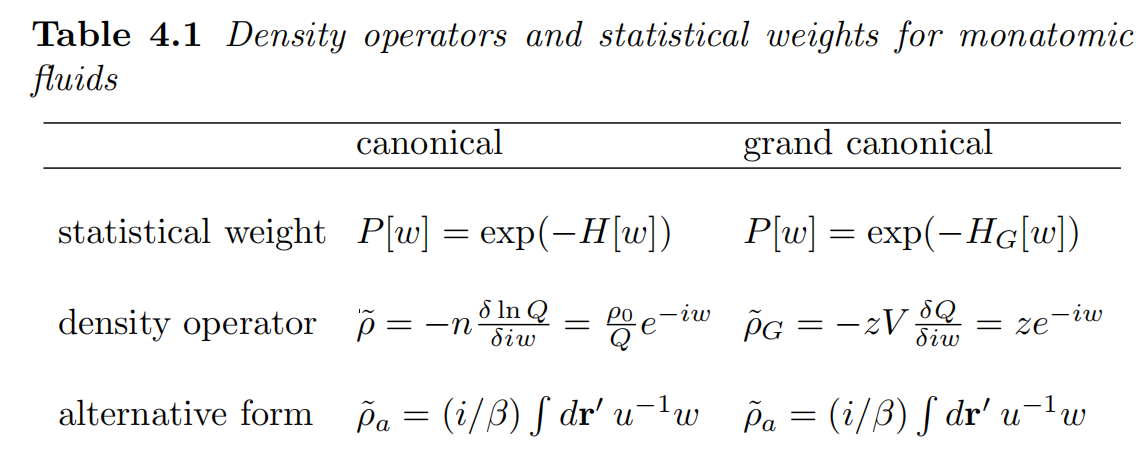
\includegraphics[width=12cm]{./figures/1.png}
	\caption{单原子流体的密度算子和统计权重}
	\label{4.1}
\end{figure}

